% THIS DOCUMENT IS TAILORED TO REQUIREMENTS FOR SCIENTIFIC COMPUTING.  IT SHOULDN'T
% BE USED FOR NON-SCIENTIFIC COMPUTING PROJECTS
\documentclass[12pt]{article}

\usepackage{amsmath, mathtools}
\usepackage{amsfonts}
\usepackage{amssymb}
\usepackage{graphicx}
\usepackage{colortbl}
\usepackage{xr}
\usepackage{hyperref}
\usepackage{longtable}
\usepackage{xfrac}
\usepackage{tabularx}
\usepackage{float}
\usepackage{siunitx}
\usepackage{booktabs}
\usepackage{caption}
\usepackage{pdflscape}
\usepackage{afterpage}
\usepackage{mathrsfs,amsmath}
\usepackage{gensymb}
\usepackage{soul,xcolor}

\usepackage{biblatex}
\addbibresource{../../refs/References.bib}

%\usepackage{refcheck}

\hypersetup{
    bookmarks=true,         % show bookmarks bar?
      colorlinks=true,       % false: boxed links; true: colored links
    linkcolor=red,          % color of internal links (change box color with linkbordercolor)
    citecolor=green,        % color of links to bibliography
    filecolor=magenta,      % color of file links
    urlcolor=cyan           % color of external links
}

\input{../Comments}
\input{../Common}

% For easy change of table widths
\newcommand{\colZwidth}{1.0\textwidth}
\newcommand{\colAwidth}{0.13\textwidth}
\newcommand{\colBwidth}{0.82\textwidth}
\newcommand{\colCwidth}{0.1\textwidth}
\newcommand{\colDwidth}{0.05\textwidth}
\newcommand{\colEwidth}{0.8\textwidth}
\newcommand{\colFwidth}{0.17\textwidth}
\newcommand{\colGwidth}{0.5\textwidth}
\newcommand{\colHwidth}{0.28\textwidth}

% Used so that cross-references have a meaningful prefix
\newcounter{defnum} %Definition Number
\newcommand{\dthedefnum}{GD\thedefnum}
\newcommand{\dref}[1]{GD\ref{#1}}
\newcounter{datadefnum} %Datadefinition Number
\newcommand{\ddthedatadefnum}{DD\thedatadefnum}
\newcommand{\ddref}[1]{DD\ref{#1}}
\newcounter{theorynum} %Theory Number
\newcommand{\tthetheorynum}{TM\thetheorynum}
\newcommand{\tref}[1]{TM\ref{#1}}
\newcounter{tablenum} %Table Number
\newcommand{\tbthetablenum}{TB\thetablenum}
\newcommand{\tbref}[1]{TB\ref{#1}}
\newcounter{assumpnum} %Assumption Number
\newcommand{\atheassumpnum}{A\theassumpnum}
\newcommand{\aref}[1]{A\ref{#1}}
\newcounter{goalnum} %Goal Number
\newcommand{\gthegoalnum}{GS\thegoalnum}
\newcommand{\gsref}[1]{GS\ref{#1}}
\newcounter{instnum} %Instance Number
\newcommand{\itheinstnum}{IM\theinstnum}
\newcommand{\iref}[1]{IM\ref{#1}}
\newcounter{reqnum} %Requirement Number
\newcommand{\rthereqnum}{R\thereqnum}
\newcommand{\rref}[1]{R\ref{#1}}
\newcounter{nfrnum} %NFR Number
\newcommand{\rthenfrnum}{NFR\thenfrnum}
\newcommand{\nfrref}[1]{NFR\ref{#1}}
\newcounter{lcnum} %Likely change number
\newcommand{\lthelcnum}{LC\thelcnum}
\newcommand{\lcref}[1]{LC\ref{#1}}
\newcounter{ucnum} %Unlikely change number
\newcommand{\ltheucnum}{LC\theucnum}
\newcommand{\ucref}[1]{UC\ref{#1}}

\usepackage{fullpage}

\newcommand{\deftheory}[9][Not Applicable]
{
\newpage
\noindent \rule{\textwidth}{0.5mm}

\paragraph{RefName: } \textbf{#2} \phantomsection
\label{#2}

\paragraph{Label:} #3

\noindent \rule{\textwidth}{0.5mm}

\paragraph{Equation:}

#4

\paragraph{Description:}

#5

\paragraph{Notes:}

#6

\paragraph{Source:}

#7

\paragraph{Ref.\ By:}

#8

\paragraph{Preconditions for \hyperref[#2]{#2}:}
\label{#2_precond}

#9

\paragraph{Derivation for \hyperref[#2]{#2}:}
\label{#2_deriv}

#1

\noindent \rule{\textwidth}{0.5mm}

}
\newcommand{\add}{\textcolor{red}}

\begin{document}
\setstcolor{red}


\title{Software Requirements Specification for \progname}
\author{\authname}
\date{\today}

\maketitle

~\newpage

\pagenumbering{roman}

\tableofcontents

~\newpage

\section*{Revision History}

\begin{tabularx}{\textwidth}{p{3cm}p{2cm}X}
\toprule {\bf Date} & {\bf Version} & {\bf Notes}\\
\midrule
Jan 23, 2025 & 1.0 & Initial Draft \\
Apr 10, 2025 & 2.0 & Final Documentation \\
\bottomrule
\end{tabularx}


~\newpage

\section{Reference Material}\label{reference material}

This section records information for easy reference.
\subsection{Table of Units}

Throughout this document SI (Syst\`{e}me International d'Unit\'{e}s) is employed
as the unit system.  In addition to the basic units, several derived units are
used as described below.  For each unit, the symbol is given followed by a
description of the unit and the SI name.
~\newline

\renewcommand{\arraystretch}{1.2}
  \noindent \begin{tabular}{l l l}
    \toprule
    \textbf{symbol} & \textbf{unit} & \textbf{SI}\\
    \midrule
    \si{\metre} & length & metre\\
    \degree & angle & degree\\
    \bottomrule
  \end{tabular}

\subsection{Table of Symbols}
The table that follows summarizes the symbols used in this document along with
their units.  The choice of symbols was made to be consistent with existing
documentation. For its definition, please refer to the Section \ref{term}.

\renewcommand{\arraystretch}{1.2}
\noindent \begin{tabular}{l l l}
\toprule
\textbf{symbol} & \textbf{unit} & \textbf{description}\\
\midrule
$I$ & None & Intensity \\
$I_{0}$ & None & Initial intensity \\
$A$ & None & Attenuation coefficient \\
$A_{max}$ & None & Highest attenuation coefficient \\
$\theta$ & \degree & Rotation degree \\
$t$ & \si{\meter} & X-ray path length \\
$\omega$ &     None       & Filter frequency variable\\
$\omega_{max}$ &     None       & Maximum filter frequency variable\\
\bottomrule
\end{tabular}\\

\subsection{Abbreviations and Acronyms}

\renewcommand{\arraystretch}{1.2}
\begin{tabular}{l l}
  \toprule
  \textbf{symbol} & \textbf{description}\\
  \midrule
  A & Assumption\\
  DD & Data Definition\\
  GD & General Definition\\
  GS & Goal Statement\\
  IM & Instance Model\\
  LC & Likely Change\\
  PS & Physical System Description\\
  R & Requirement\\
  SRS & Software Requirements Specification\\
  \progname{} & Filter back projection for CT image reconstruction\\
  TM & Theoretical Model\\
  \bottomrule
\end{tabular}\\

\newpage

\section{Introduction} \label{introduction}
%% Problem domain
Image reconstruction is the process of turning raw data collected by the
detectors into image data which can be viewed on a screen. \add{The most common
  CT image reconstruction method is back-projection. However, there is a large
  amount of noise in this method which result a blur reconstructed image
  \cite{Beatty2012}.} \st{Both raw data and image data can be manipulated in
  different ways to create images with differing properties. The most
  rudimentary process of turning raw data into image data is called
  back-projection. This is the process of mathematically mapping the attenuation
  pathway at every angle measured through a scan to locate where in a patient
  attenuation is occurring. However, even if the number of back-projection is
  increased (say to 1000 directions), there is still a large amount of noise
  blurring the recreate image. As it turns out, no matter how many directions we
  try to backproject in, it is not able to perfectly recreate our image using
  the back-projection. For this process to be at all useful, it is necessary to
  derive a way to filter out some of the noise the back-projection formula seems
  to create in our picture and get a smoother representation of our object.}
\add{\progname aims to filter out the noise and provide a clearer reconstructed CT image for
  researchers by applying filter techniques during the back-projection. This
  tool also provide a simulation to sinogram for researchers who want to
  simulate the CT detector behavior(collect the intensity and generate the
  sinogram data) given the image of organ when they can not get the data from patients.}

%% Roadmap for what subsection to expect in the Introduction
The following subsections will outline the primary aspects of SRS,
ensuring clarity in understanding the \progname purpose, scope, and organization of the
system requirements.

\subsection{Purpose of Document}
This document serves to guide software developers and researchers in
understanding the technical challenges and requirements involved in the project.
It aims to facilitate effective communication between team members and domain
experts, ensuring a correct and efficient implementation of Filter
Back-projection (FBP) method for CT image reconstruction.

Additionally, this document serves as a reference for users of the software to
understand its capabilities, limitations, and assumptions. It also acts as a
valuable resource for future maintenance, and verification of the implemented
methods, ensuring long-term usability and reliability of the software.

\subsection{Scope of Requirements}
This project focuses on implementing FBP methods for CT image reconstruction,
with simplifications applied to manage the complexity of real-world challenges.
The scope is constrained to reconstructing 2D images from raw projection data
obtained through ideal scanning conditions. It excludes considerations such as
non-ideal scanner geometries, variations in detector sensitivity, or artifacts
caused by motion during scanning.

The implementation will primarily address noise reduction and basic filtering,
without delving into advanced techniques like iterative reconstruction or
machine learning-based enhancements. The software assumes uniform spacing
between projection angles and consistent image resolution.

\subsection{Characteristics of Intended Reader} \label{sec_IntendedReader}
The intended readers of this document are individuals involved in the development,
review, and maintenance of the FBP tool for CT image reconstruction. These
readers are expected to have a basic understanding of computed tomography
principles and image processing techniques such as Fourier transforms, Random
transforms, linear algebra and Python.

\subsection{Organization of Document}
The introduction section (Section~\ref{introduction}) provides an overview of
the project, including the purpose, scope, and intended audience for this
document. The General System Description (Section~\ref{general description}) outlines
the context and high-level requirements of the system. Detailed problem
definitions, theoretical foundations, and specific system functionalities are
described in the Specific System Description (Section~\ref{specific description}). The
Requirements section (Section~\ref{requirement}) specifies both functional
and non-functional requirements. The document concludes with an overview of
potential changes and their implications for future development.

\section{General System Description} \label{general description}

This section provides general information about the system.  It identifies the
interfaces between the system and its environment, describes the user
characteristics and lists the system constraints.

\subsection{System Context}
\begin{figure}[h!]
\begin{center}
 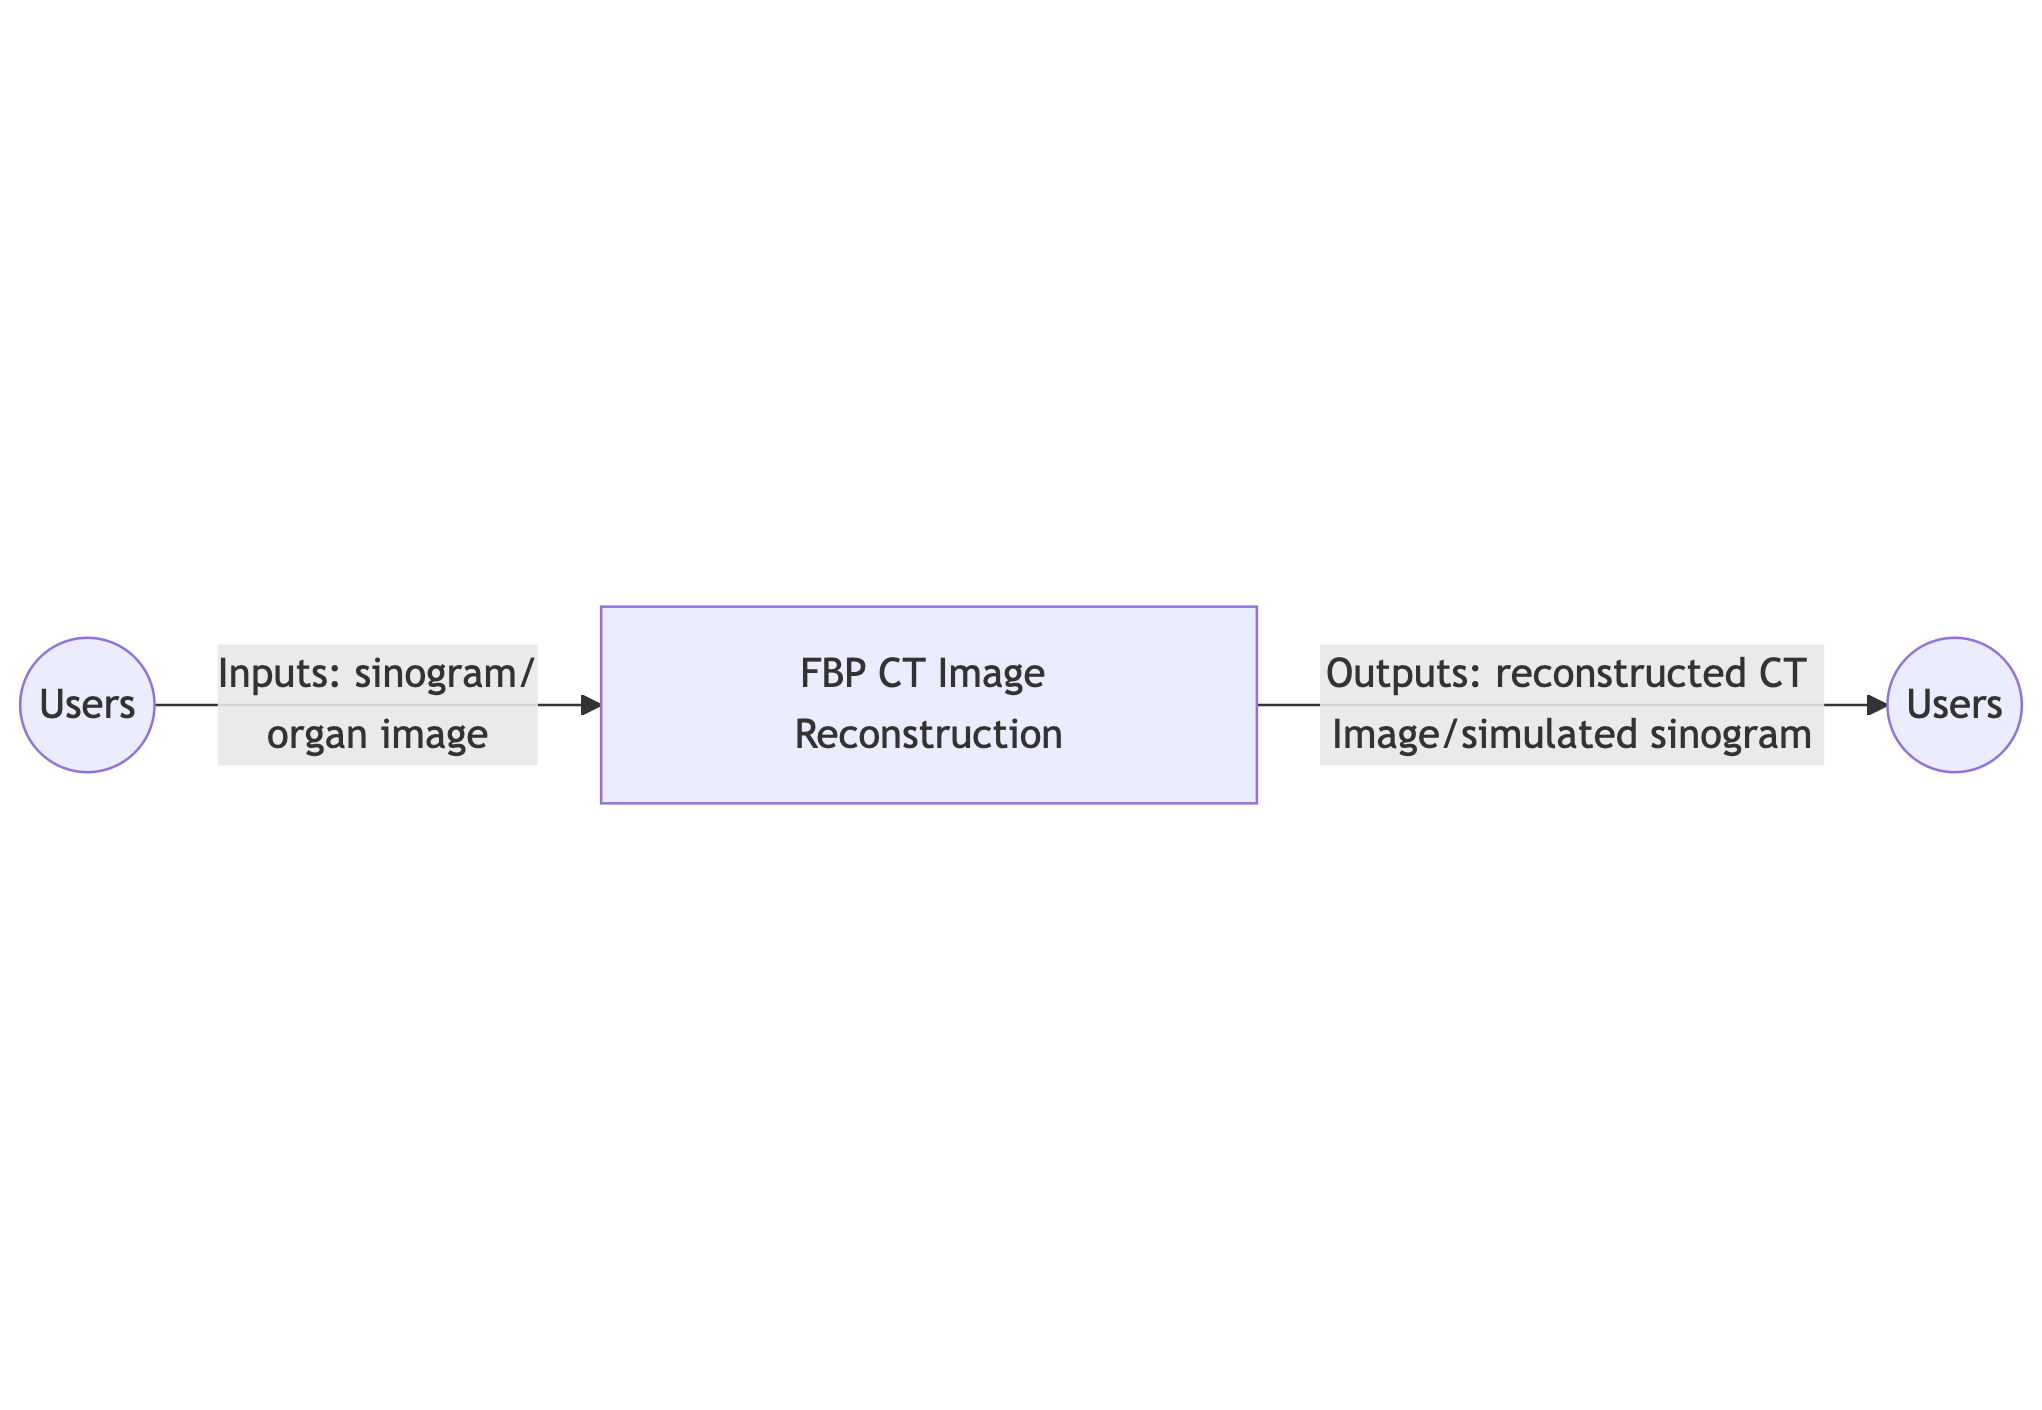
\includegraphics[width=0.9\textwidth]{SysConfig.png}
\caption{System Context}
\label{Fig_SystemContext}
\end{center}
\end{figure}


\begin{itemize}
\item User Responsibilities:
\begin{itemize}
\item Provide X-ray projection data in a standardized format.
\item Select appropriate filtering methods.
\item Interpret and analyze the reconstructed images.
\end{itemize}
\end{itemize}


\begin{itemize}
\item Software Responsibilities:
\begin{itemize}
\item Validate input data to ensure compatibility with the processing pipeline.
\item Apply transformations and filtering to extract attenuation values.
\item Generate reconstructed images based on back-projection techniques.
\item Ensure computational efficiency by leveraging optimized libraries.
\end{itemize}
\end{itemize}

\subsection{User Characteristics} \label{SecUserCharacteristics} The primary
users of this tool for CT image reconstruction are individuals with a background
in computed tomography, image processing, and numerical methods. They are
expected to have at least an undergraduate-level understanding of calculus,
linear algebra, and Fourier transforms, as these concepts are fundamental to the
reconstruction process. Familiarity with Radon transforms, filtering techniques
(such as Ramp and Shepp-Logan filters) \st{, and Python programming} is also required
to effectively use and modify the system. Users may include medical imaging
researchers, software engineers developing CT reconstruction algorithms, and
graduate students studying image processing techniques.

\subsection{System Constraints}
This tool must operate within specific system constraints to ensure
compatibility, performance, and usability. \add{The \progname \space is limited
  by the trade-off between noise suppression and edge preservation imposed by
  the choice of frequency-domain filters (e.g., Ramp, Shepp-Logan, Hamming).
  Additionally, the system requires sufficient computational resources to
  perform Fourier transforms and back-projection efficiently, especially for
  high-resolution images.}
\st{The software must be implemented in Python, leveraging libraries
  such as NumPy, SciPy, and scikit-image for numerical computations and image
  processing. It must support grayscale 2D images with a fixed resolution to
  ensure uniform data
  processing.\\

Additionally, the system should be optimized to run efficiently on
standard computing hardware, avoiding dependencies on specialized GPU
acceleration. Furthermore, the input data format must conform to a standardized
structure, ensuring that projection data and filtering parameters align with the
expected mathematical models.
}
\section{Specific System Description} \label{specific description} This section
first presents the problem description, which gives a high-level view of the
problem to be solved in \progname{}. This is followed by the solution
characteristics specification, which presents the assumptions, theories,
definitions and finally the instance models.

\subsection{Problem Description} \label{Sec_pd}

\progname{} is a tool designed to address the issue of blurry CT reconstructed
images resulting from simple back projection.

\subsubsection{Terminology and  Definitions} \label{term}
This subsection provides a list of terms that are used in the subsequent
sections and their meaning, with the purpose of reducing ambiguity and making it
easier to correctly understand the requirements:

\begin{center}
\begin{longtable}{|l|p{10cm}|}
  \caption{Terminology and Definitions.\label{long}}\\

\hline
 \multicolumn{2}{|c|}{Begin of Table}\\
 \hline
 Terminology & Definitions\\
 \hline
 \endfirsthead

 \hline
 \multicolumn{2}{|c|}{Continuation of Table \ref{long}}\\
 \hline
 Terminology & Definitions\\
 \hline
 \endhead

 \hline
 \endfoot

 \hline
 \multicolumn{2}{| c |}{End of Table}\\
 \hline\hline
 \endlastfoot

  Intensity & The measure of brightness or signal strength in an image, representing the amount of X-ray energy detected after passing through an object. In CT images, intensity values correspond to the attenuation of X-rays by different tissues.\\
  \hline

  Attenuation Coefficient A&  measure of how much an X-ray beam is reduced in intensity as it passes through a material, depending on the material's density and composition.\\
  \hline

  Radon Transform (Sinogram) & A mathematical transformation that converts an image from the spatial domain to the projection domain by integrating values along specific directions.\\
  \hline

  Fourier Transform & Converting sinogram from the projection domain to the frequency domain.\\
  \hline

  Inverse Fourier Transform & Converting the projection data back to the spatial projection domain.\\
  \hline

  Fourier domain & A representation of signals in the frequency domain, where CT images can be reconstructed using Fourier transforms to analyze spatial frequency components.\\
  \hline

  Spatial domain & The domain in which an image is represented in terms of pixel intensities, as opposed to the frequency domain.\\
  \hline

  Projection domain & The projection domain is a mathematical representation of an object's line integrals taken from multiple angles, rather than its direct spatial structure.\\
  \hline

  Low-pass filter & A filter that allows low-frequency components to pass through while reducing high-frequency noise, commonly used in image smoothing.\\
  \hline

  High-pass filter & A filter that enhances high-frequency components while attenuating low-frequenggcy signals, often used to sharpen images or enhance edges.\\
  \hline

  Back Projection (BP) & Maps filtered projections to reconstruct the image in spatial domain.\\
  \hline

  Filter Back Projection (FBP) & A widely used image reconstruction technique in CT that improves upon simple back projection by applying a filtering step in the frequency domain. This enhances image quality by reducing blurring and artifacts.\\
  \hline

  Monochromatic X-rays & They have a single photon energy without beam hardening artifacts.\\
  \hline

  Polychromatic X-rays & They contain a range of photon energies, causing beam hardening, where lower-energy photons are absorbed more, making attenuation non-linear and requiring corrections.\\
  \hline
\end{longtable}
\end{center}

\subsubsection{Physical System Description} \label{sec_phySystDescrip}
The physical system of \progname{}, includes the following elements:

\begin{description}
\item[PS1:] X-Ray Source \hfill \\
  The CT scanner's X-ray tube emits X-ray beams that pass through the object being scanned.

\item[PS2:] Scanned Object (Patient or Sample) \hfill \\
  \st{he} \add{The} physical object being imaged, which could be a biological tissue, industrial material, or any sample placed in the CT scanner.

\item[PS3:] X-Ray Detectors \hfill \\
  A ring or array of sensors that measure the intensity of X-rays after passing through the scanned object.

%\item[PS4:] Projection Data \hfill \\
  %A collection of intensity values recorded by detectors for multiple angles
%
%\item[PS5:] Reconstructed Image \hfill \\
  %Result of numerical processing transforms raw projection data into a cross-sectional image.
\end{description}

%\plt{A figure here makes sense for most SRS documents}

% \begin{figure}[h!]
% \begin{center}
% %\rotatebox{-90}
% {
%  \includegraphics[width=0.5\textwidth]{<FigureName>}
% }
% \caption{\label{<Label>} <Caption>}
% \end{center}
% \end{figure}

\subsubsection{Goal Statements}
\noindent Given a set of raw intensity data measured by a CT scanner detector array, the goal statements are:

\begin{itemize}

\item[GS\refstepcounter{goalnum}\thegoalnum \label{G1}:] Implement High-Pass
  Filtered Back Projection to reconstruct a sharper edge CT image.

\item[GS\refstepcounter{goalnum}\thegoalnum \label{G2}:] Implement Low-Pass
  Filtered Back Projection to reconstruct an overall smooth CT image.
\end{itemize}

\subsection{Solution Characteristics Specification}
\begin{figure}[H]
  \includegraphics[scale=0.9]{RelationsBetweenTM_GD_IM_DD_A.pdf}
\end{figure}

The instance models that govern \progname{} are presented in
Subsection~\ref{sec_instance}.  The information to understand the meaning of the
instance models and their derivation is also presented, so that the instance
models can be verified.


\subsubsection{Assumptions} \label{sec_assumpt}
This section simplifies the original problem and helps in developing the
theoretical model by filling in the missing information for the physical system.
The numbers given in the square brackets refer to the theoretical model [TM],
general definition [GD], data definition [DD], instance model [IM], or likely
change [LC], in which the respective assumption is used.

\begin{itemize}
\item[A\refstepcounter{assumpnum}\theassumpnum \label{A1}:] The Ramp and
  Shepp-Logan filters are assumed to be representative of high-pass and low-pass
  filtering techniques. [TM\ref{TM4}, TM\ref{TM5}, IM\ref{IM1}, IM\ref{IM2}]

\item[A\refstepcounter{assumpnum}\theassumpnum \label{A2}:] The system assumes that
  the CT scanner uses a monochromatic (single-energy) X-ray source to avoid beam
  hardening artifacts. In reality, CT scanners use polychromatic X-rays, but for
  mathematical simplicity, this assumption is made. [DD\ref{DD1}]
\end{itemize}

\subsubsection{Theoretical Models}\label{sec_theoretical}
This section focuses on the general equations and laws that \progname{} is based
on.
~\newline

\noindent
\begin{minipage}{\textwidth}
	\renewcommand*{\arraystretch}{1.5}
	\begin{tabular}{| p{\colAwidth} | p{\colBwidth}|}
   \hline
   Number& TM\refstepcounter{theorynum}\thetheorynum \label{TM1}\\
   \hline
   Label&\bf Log Transformation\\
   \hline
   Equation& $y = \log_{b}(x) \Longleftrightarrow b^y = x$ \\
   \hline
	  Description & It expresses the fundamental relationship between logarithms and exponents, showing their equivalence. \\
	  \hline
    Note & None\\
    \hline
    Source & None\\
    \hline
    Ref.\ By & GD\ref{GD1} \\
    \hline
	\end{tabular}
\end{minipage}\\

~\newline
\noindent
\begin{minipage}{\textwidth}
	\renewcommand*{\arraystretch}{1.5}
	\begin{tabular}{| p{\colAwidth} | p{\colBwidth}|}
   \hline
   Number& TM\refstepcounter{theorynum}\thetheorynum \label{TM2}\\
   \hline
   Label&\bf Randon Transform \\
   \hline
   Equation& \add{\[Rf(s, z) = \int_{-\infty}^{\infty} f(x(z), y(z)) \, dz\] with \[(x(z),y(z)) = ((z\sin\alpha + s\cos\alpha), (-z\cos\alpha + s\sin\alpha))\]} \\
   \hline
	  Description & The $Rf(t, \theta)$ represents the projection data given the detected intensity data. Where:
                  \begin{itemize}
                  \item $f(x(z),y(z))$ represents the original function describing the
                    intensity absortion coefficient alone the path. In CT image
                    reconstruction, it is attenuation coefficient.
                  \item The result, $Rf(x, z)$, provides a function of:
                    \begin{itemize}
                    \item $s$: The perpendicular distance from the origin to the
                      projection line.
                    \item $z$: The projection distance used during scanning.
                    \end{itemize}
                  \end{itemize} \\
	  \hline
    Note & None\\
    \hline
    Source & \cite{Beatty2012}\\
    \hline
    Ref.\ By & TM\ref{TM3}, IM\ref{IM1}, IM\ref{IM2} \\
    \hline
	\end{tabular}
\end{minipage}\\

~\newline
\begin{minipage}{\textwidth}
	\renewcommand*{\arraystretch}{1.5}
	\begin{tabular}{| p{\colAwidth} | p{\colBwidth}|}
    \hline
    Number& TM\refstepcounter{theorynum}\thetheorynum \label{TM3}\\
    \hline
    Label&\bf Back Projection \\
    \hline
    Equation& \add{\[f = R^{-1}f(s, z)\]} \\
    \hline
	  Description & The Back Projection, also known as the Inverse Radon Transform, is a technique used to reconstruct an image by solving the inverse problem of the randon function [TM\ref{TM2}]. It is widely applied in CT and other imaging techniques to recover the original function from its Radon transform.\\
	  \hline
    Note & None\\
    \hline
    Source & \cite{Beatty2012}\\
    \hline
    Ref.\ By & IM\ref{IM1}, IM\ref{IM2}, GD\ref{GD1} \\
    \hline
	\end{tabular}
\end{minipage}\\

~\newline
\begin{minipage}{\textwidth}
	\renewcommand*{\arraystretch}{1.5}
	\begin{tabular}{| p{\colAwidth} | p{\colBwidth}|}
    \hline
    Number& TM\refstepcounter{theorynum}\thetheorynum \label{TM4}\\
    \hline
    Label&\bf Ramp Filter (high pass filter) \\
    \hline
    Equation& \[H(\omega) = |\omega|\] \\
    \hline
	  Description & The Ramp filter belongs to the high pass filter [A\ref{A1}]. It helps to counteract the blurring introduced by simple back projection, improving image sharpness and accuracy.
                  \begin{itemize}
                  \item $H(\omega)$ represents the Ramp Filter, it is an 1D array with length same as the number of projection.
                  \item \add{$|\omega|$ is absolute value that represent angular frequency.}
                  \end{itemize} \\
	  \hline
    Note & None\\
    \hline
    Source & \cite{Beatty2012}\\
    \hline
    Ref.\ By & IM\ref{IM1}\\
    \hline
	\end{tabular}
\end{minipage}\\


~\newline
\begin{minipage}{\textwidth}
	\renewcommand*{\arraystretch}{1.5}
	\begin{tabular}{| p{\colAwidth} | p{\colBwidth}|}
    \hline
    Number& TM\refstepcounter{theorynum}\thetheorynum \label{TM5}\\
    \hline
    Label&\bf Shepp-Logan Filter (low pass filter) \\
    \hline
    Equation& \[S(\omega) = |\omega| \cdot sinc(\frac{\omega}{2\omega_{max}})\] \add{where \[sinc(x) = \frac{\sin (\pi x)}{\pi x}\]} \\
    \hline
	  Description & The Shepp-Logan filter is a modified version of the Ramp Filter used in low-pass filter [A\ref{A1}] for CT image reconstruction. It helps reduce noise by attenuating high frequencies smoothly.
                  \begin{itemize}
                  \item $S(\omega)$ represents the Shepp-Logan Filter. It is an 1D array with the length same as the number of projections.
                  \item $\omega$ is the frequency variable.
                  \item $\omega_{max}$ is the maximum frequency (cutoff frequency).
                  \item $sinc(x)$ is the sinc function,
                    which introduces smooth attenuation of high frequencies.
                  \end{itemize} \\
	  \hline
    Note & None\\
    \hline
    Source & \cite{Beatty2012}\\
    \hline
    Ref.\ By & IM\ref{IM2}\\
    \hline
	\end{tabular}
\end{minipage}\\


~\newline
\begin{minipage}{\textwidth}
	\renewcommand*{\arraystretch}{1.5}
	\begin{tabular}{| p{\colAwidth} | p{\colBwidth}|}
    \hline
    Number& TM\refstepcounter{theorynum}\thetheorynum \label{TM6}\\
    \hline
    Label&\bf Fourier Transform\\
    \hline
    Equation& \[F(\omega) = \mathcal{F} \{f(\omega)\} = \int_{-\infty} ^{\infty} f(\omega) e^{-j \omega x}\, d\omega\] \\
    \hline
	  Description & Fourier Transform ($\mathcal{F} \{f(\omega)\}$) Converts a function from the spatial domain to the frequency domain.
                  \begin{itemize}
                  \item $F(\omega)$  is the function in the frequency domain.
                  \item $\omega$ is the frequency variable.
                  \item $f(\omega)$ is the function in the spatial domain.
                  \item $e^{-j \omega x}$ represents the complex exponential basis
                    function (where $j = \sqrt{-1}$).
                  \end{itemize} \\
	  \hline
    Note & None\\
    \hline
    Source & \cite{Beatty2012}\\
    \hline
    Ref.\ By & IM\ref{IM1}, IM\ref{IM2}\\
    \hline
	\end{tabular}
\end{minipage}\\


~\newline
\begin{minipage}{\textwidth}
	\renewcommand*{\arraystretch}{1.5}
	\begin{tabular}{| p{\colAwidth} | p{\colBwidth}|}
    \hline
    Number& TM\refstepcounter{theorynum}\thetheorynum \label{TM7}\\
    \hline
    Label&\bf Inverse Fourier Transform\\
    \hline
    Equation& \[F(\omega) = \mathcal{F}^{-1} \{F(\omega)\} = \frac{1}{2\pi}\int_{-\infty} ^{\infty} F(\omega) e^{j \omega x}\, d\omega\] \\
    \hline
	  Description & Inverse Fourier Transform ($\mathcal{F}^{-1} \{F(\omega)\}$) Converts a function from the frequency domain back to the spatial domain.
                  \begin{itemize}
                  \item $F(\omega)$ is the function in the frequency domain.
                  \item $\omega$ is the frequency variable.
                  \item $f(\omega)$ is the function in the spatial domain.
                  \item $e^{j \omega x}$ represents the inverse transformation basis.
                  \end{itemize} \\
	  \hline
    Note & None\\
    \hline
    Source & \cite{Beatty2012}\\
    \hline
    Ref.\ By & IM\ref{IM1}, IM\ref{IM2}\\
    \hline
	\end{tabular}
\end{minipage}\\

~\newline

\subsubsection{General Definitions}\label{sec_gendef}
This section collects the laws and equations that will be used in building the
instance models.

\noindent
\begin{minipage}{\textwidth}
	\renewcommand*{\arraystretch}{1.5}
	\begin{tabular}{| p{\colAwidth} | p{\colBwidth}|}
    \hline
    Number& GD\refstepcounter{defnum}\thedefnum \label{GD1}\\
    \hline
    Label&\bf Intensity data projection\\
    \hline
    SI Units & None\\
    \hline
    Equation& $P(t,\theta) = -\ln(\frac{I(t,\theta)}{I_0}) = \int_{x-ray path} f(x,y) ds = Rf(t, \theta)$ \\
    \hline
	  Description & Taking the logarithm to linearize the exponential relationship,
converting the intensity data[DD\ref{DD1}] from spacial domain into projection domain. This
transformation allows the Radon Transform [TM\ref{TM2}] to directly represent line
integrals of the attenuation coefficient [DD\ref{DD2}].
    $P(t,\theta) = -\ln(\frac{I(t,\theta)}{I_0})$ is the value used as an input of back projection. [TM\ref{TM3}] \\
    \hline
    Source & None\\
    \hline
    Ref.\ By & IM\ref{IM1}, IM\ref{IM2}\\
    \hline
	\end{tabular}
\end{minipage}\\

\subsubsection*{Detailed derivation of converting intensity from spatial domain to
  projection domain}

The X-ray intensity [DD\ref{DD1}] after passing through an object follows:

\begin{equation}
    I(t, \theta) = I_0 e^{-\int_{\textnormal{x-ray path}} f(x,y) ds}
\end{equation}

where:
\begin{itemize}
    \item \( I(t, \theta) \) is the measured intensity at detector position \( t \) for angle \( \theta \),
    \item \( I_0 \) is the initial X-ray intensity,
    \item \( f(x,y) \) is the attenuation coefficient of the object, [DD\ref{DD2}]
    \item The integral sums the attenuation along the X-ray path \( ds \).
\end{itemize}

To linearize this equation, we take the natural logarithm on both sides:

\begin{equation}
    \ln I(t, \theta) = \ln I_0 - \int_{\textnormal{x-ray path}} f(x,y) ds
\end{equation}

Rearranging the equation:

\begin{equation}
    -\ln \left( \frac{I(t, \theta)}{I_0} \right) = \int_{\textnormal{x-ray path}} f(x,y) ds
\end{equation}

Thus, defining the projection data \( P(t, \theta) \):

\begin{equation}
    P(t,\theta) = -\ln(\frac{I(t,\theta)}{I_0})
\end{equation}

This equation represents the Radon Transform [TM\ref{TM2}], which maps the
intensity from spatial domain $I(t, \theta)$ into the projection domain $P(t, \theta)$.


~\newline

\subsubsection{Data Definitions}\label{sec_datadef}
This section collects and defines all the data types needed to document the
models.
~\newline
\noindent
\begin{minipage}{\textwidth}
	\renewcommand*{\arraystretch}{1.5}
	\begin{tabular}{| p{\colAwidth} | p{\colBwidth}|}
    \hline
    Number& DD\refstepcounter{datadefnum}\thedatadefnum \label{DD1}\\
    \hline
    Label&\bf Intensity Data\\
    \hline
    Symbol& $I(t,\theta)$\\
    \hline
    SI Units& None\\
    \hline
    Equation& $I(t,\theta) = I_0e^{-\int_{x-ray path} f(x, y) ds}$ \\
    \hline
	  Description & This projection data represents the attenuated linear X-ray [A\ref{A2}] intensity after passing through the object. Where:
                  \begin{itemize}
                  \item $I(t,\theta)$ is the measured intensity at detector position.
                  \item $I_0$ is the initial intensity.
                  \item $f(x,y)$ is the unknown attenuation coefficient [DD\ref{DD2}].
                  \item s: The length of x-ray path. The integral sums the attenuation along the X-ray path.
                  \end{itemize} \\
    \hline
    Source & \cite{Beatty2012}\\
    \hline
    Ref.\ By & GD\ref{GD1}, IM\ref{IM1}, IM\ref{IM2}\\
    \hline
	\end{tabular}
\end{minipage}\\

~\newline
\noindent
\begin{minipage}{\textwidth}
	\renewcommand*{\arraystretch}{1.5}
	\begin{tabular}{| p{\colAwidth} | p{\colBwidth}|}
    \hline
    Number& DD\refstepcounter{datadefnum}\thedatadefnum \label{DD2}\\
    \hline
    Label&\bf Attenuation Coefficient\\
    \hline
    Symbol& $A(x, y)$\\
    \hline
    SI Units& None\\
    \hline
    Equation& $A(x, y) = f(x,y)$ \\
    \hline
	  Description & It denoted as $f(x,y)$, represents the degree to which X-ray
intensity [DD\ref{DD1}] is reduced as it passes through a material at a given
location $(x,y)$. It quantifies the fraction of the X-ray beam that is absorbed
or scattered per unit distance and is a fundamental property used in CT image
reconstruction to characterize tissue composition.\\
    \hline
    Source & \cite{Beatty2012}\\
    \hline
    Ref.\ By & IM\ref{IM1}, IM\ref{IM2}, TM\ref{TM2}, TM\ref{TM3}, GD\ref{GD1}\\
    \hline
	\end{tabular}
\end{minipage}\\

\subsubsection{Data Types}\label{sec_datatypes}
This section collects and defines all the data types needed to document the
models. In this system, it isn't necessary, since the inputs and outputs are
straightforward types, like reals, integers, and sequences of reals and
integers. Please refer to IM\ref{IM1} and IM\ref{IM2}.

\subsubsection{Instance Models} \label{sec_instance}
This section transforms the problem defined in Section~\ref{Sec_pd} into
one which is expressed in mathematical terms. It uses concrete symbols defined
in Section~\ref{sec_datadef} to replace the abstract symbols in the models
identified in Sections~\ref{sec_theoretical}.\\

The goals GS\ref{G1} are solved by IM\ref{IM1} and he goals GS\ref{G2} are solved by IM\ref{IM2}.
~\newline

% IM1
\noindent
\begin{minipage}{\textwidth}
	\renewcommand*{\arraystretch}{1.5}
	\begin{tabular}{| p{\colAwidth} | p{\colBwidth}|}
    \hline
    Number& IM\refstepcounter{instnum}\theinstnum \label{IM1}\\
    \hline
    Label&\bf Ramp filter back projection to reconstruct Attenuation Coefficient \\
    \hline
    Input& \begin{itemize}
            \item $I(t,\theta)$: A 2D array (M * N) with value measured X-ray intensity where:
             \begin{itemize}
               \item M: Number of detector positions t.
               \item N: Number of projection angles $\theta$.
             \end{itemize}
            \item $\theta$: projection angles in degree or radium.
            \item $H(\omega)$: \add{The ramp filter in TM[\ref{TM4}]}\st{1D array of filtering variable representing the high-pass filter}.
           \end{itemize} \\
    \hline
    Equation& \[A(x,y) = \frac{1}{\pi} \int_{0}^{\pi} \mathcal{F}^{-1} {\mathcal{F} [-\ln{\frac{I(t,\theta)}{I_0}} \cdot H(\omega)]}\] \\
    \hline
    Output& $A(x,y)$: 2D array (P × P), where P is the image resolution. \\
    \hline
	  Description & This instance model describes the Filtered Back Projection, which reconstructs the $A(x,y)$ from projection data. The method consists of:
                  \begin{itemize}
                  \item Log transformation of intensity data $I(t,\theta)$ to obtain
                    projection data $P(t,\theta)$. [DD\ref{DD1}]
                  \item Radon Transform interpretation, where $P(t,\theta) = Rf(t,\theta)$. [GD\ref{GD1}]
                  \item Fourier filtering with Ramp filter $H(\omega)$ to enhance
                    reconstruction accuracy. [TM\ref{TM4}, TM\ref{TM6}, TM\ref{TM7}]
                  \item Back Projection over all projection angles $\theta$ to
                    reconstruct the final image. [TM\ref{TM3}, DD\ref{DD2}]
                  \end{itemize} \\
    \hline
    Source & \cite{Beatty2012}\\
    \hline
    Ref.\ By & None \\
    \hline
	\end{tabular}
\end{minipage}\\


% IM2
\noindent
\begin{minipage}{\textwidth}
	\renewcommand*{\arraystretch}{1.5}
	\begin{tabular}{| p{\colAwidth} | p{\colBwidth}|}
    \hline
    Number& IM\refstepcounter{instnum}\theinstnum \label{IM2}\\
    \hline
    Label&\bf Shepp-Logan back projection to reconstruct Attenuation Coefficient \\
    \hline
    Input&
           \begin{itemize}
           \item $I(t,\theta)$: 2D array (M * N) with value measured X-ray intensity where:
             \begin{itemize}
             \item M: Number of detector positions t.
             \item N: Number of projection angles $\theta$.
             \end{itemize}
            \item $\theta$: projection angles in degree.
            \item $S(\omega)$: 1D array of filtering variable representing the low-pass filter.
           \end{itemize} \\
    \hline
    Equation& $A(x,y) = \frac{1}{\pi} \int_{0}^{\pi} \mathcal{F}^{-1} {\mathcal{F} [-\ln{\frac{I(t,\theta)}{I_0}} \cdot S(\omega)]}$ \\
    \hline
    Output& $A(x,y)$: 2D array (P × P), where P is the image resolution. \\
    \hline
	  Description & This instance model describes the Filtered Back Projection, which reconstructs the $A(x,y)$ from projection data. The method consists of:
                  \begin{itemize}
                  \item Log transformation of intensity data $I(t,\theta)$ to obtain
                    projection data $P(t,\theta)$. [DD\ref{DD1}]
                  \item Radon Transform interpretation, where $P(t,\theta) = Rf(t,\theta)$. [GD\ref{GD1}]
                  \item Fourier filtering with Shepp-Logan filter $S(\omega)$ to enhance
                    reconstruction accuracy. [TM\ref{TM5}, TM\ref{TM6}, TM\ref{TM7}]
                  \item Back Projection over all projection angles $\theta$ to
                    reconstruct the final image. [TM\ref{TM3}, DD\ref{DD2}]
                  \end{itemize} \\
    \hline
    Source & \cite{Beatty2012}\\
    \hline
    Ref.\ By & None \\
    \hline
	\end{tabular}
\end{minipage}\\

%~\newline

\subsubsection*{Derivation of Filter Back Projection}
The Filtered Back Projection (FBP) reconstructs an image from X-ray
projections by first applying a log transformation to convert intensity
measurements into projection data. The Fourier Transform is then used to filter
the projections with a ramp or shepp-logan filter, which enhances high-frequency
details. The filtered projections are then transformed back using the Inverse
Fourier Transform. Finally, integration over all projection angles $\theta$ performs the back-projection, reconstructing the $A(x,y)$.

\subsubsection{Input Data Constraints} \label{sec_DataConstraints}

Table~\ref{TblInputVar} shows the data constraints on the input output
variables.  The column for physical constraints gives the physical limitations
on the range of values that can be taken by the variable.  The column for
software constraints restricts the range of inputs to reasonable values.  The
software constraints will be helpful in the design stage for picking suitable
algorithms.  The constraints are conservative, to give the user of the model the
flexibility to experiment with unusual situations.  The column of typical values
is intended to provide a feel for a common scenario.  The uncertainty column
provides an estimate of the confidence with which the physical quantities can be
measured.  This information would be part of the input if one were performing an
uncertainty quantification exercise.

The specification parameters in Table~\ref{TblInputVar} are listed in
Table~\ref{TblSpecParams}.

\begin{table}[!h]
  \caption{Input Variables} \label{TblInputVar}
  \renewcommand{\arraystretch}{1.2}
\noindent \begin{longtable*}{l l l l c}
  \toprule
  \textbf{Var} & \textbf{Physical Constraints} & \textbf{Software Constraints} &
                             \textbf{Typical Value} & \textbf{Uncertainty}\\
  \midrule
  $I(t,\theta)$ & $I(t,\theta) > 0$ & $0 \leq I(t,\theta) \leq I_0$ & None & 5\%\\
  \midrule
  $H(\omega)$ & Bandwidth-limit & frequency domain & None & None\\
  \midrule
  $S(\omega)$ & Bandwidth-limit & frequency domain & None & None\\
  \midrule
  $\theta$ & $0\degree \leq \theta \leq 180\degree$ & discrete angles & None & None \\
  \\
  \bottomrule
\end{longtable*}
\end{table}

\begin{table}[!h]
\caption{Specification Parameter Values} \label{TblSpecParams}
\renewcommand{\arraystretch}{1.2}
\noindent \begin{longtable*}{l l}
  \toprule
  \textbf{Var} & \textbf{Value} \\
  \midrule
  $I_0$ & 1 \\
  \bottomrule
\end{longtable*}
\end{table}

\subsubsection{Properties of a Correct Solution} \label{sec_CorrectSolution}

\noindent
A correct Filtered Back Projection reconstruction must adhere to physical
correctness and computational stability. \st{The reconstructed image should preserve
the total attenuation observed in the sinogram, ensuring consistency with the
projection data.} Additionally, the attenuation values must remain non-negative,
as negative attenuation is not physically meaningful. The reconstruction must
also respect constraints derived from the X-ray attenuation model, ensuring
values stay within a reasonable range.

A sample table is shown in Table~\ref{TblOutputVar}

\begin{table}[!h]
\caption{Output Variables} \label{TblOutputVar}
\renewcommand{\arraystretch}{1.2}
\noindent \begin{longtable*}{l l}
  \toprule
  \textbf{Var} & \textbf{Physical Constraints} \\
  \midrule
  $A(x,y)$ & $0 \leq A(x,y) \leq A_{max}$\\
  \bottomrule
\end{longtable*}
\end{table}
$A_{max}$ depends on the highest attenuation material in the scan.
\section{Requirements} \label{requirement}
This section provides the functional requirements, the business tasks that the
software is expected to complete, and the nonfunctional requirements, the
qualities that the software is expected to exhibit.

\subsection{Functional Requirements}

\noindent \begin{itemize}

\item[R\refstepcounter{reqnum}\thereqnum \label{R1}:] \add{The system should
    provide a CT detector simulation to generate sinograms given images for reconstruction.}\st{The system must accept a
  grayscale 2D input image, apply the Radon Transform to generate projection
  data, and ensure that intensity values are normalized between 0 and 1} (from
  IM\ref{IM1} and IM\ref{IM2}).

\item[R\refstepcounter{reqnum}\thereqnum \label{R2}:] The system must allow users
  to select a filtering method, choosing between the \add{Hann, Hamming}Ramp and Shepp-Logan
  filters. (from IM\ref{IM1} and IM\ref{IM2})
\item[R\refstepcounter{reqnum}\thereqnum \label{R3}:] The system must perform the
  back-projection over all projection angles to reconstruct the attenuation
  coefficient after filtering (from IM\ref{IM1} and IM\ref{IM2}).

%\item[R\refstepcounter{reqnum}\thereqnum \label{R4}:] The reconstructed attenuation
%  values must be non-negative and consistent with input projections.
\end{itemize}

\subsection{Nonfunctional Requirements}
\noindent \begin{itemize}

\item[NFR\refstepcounter{nfrnum}\thenfrnum \label{NFR_Accuracy}:]
  \textbf{Accuracy} The reconstructed attenuation values must have an error margin
  within tolerance compared to the ground truth.

\item[NFR\refstepcounter{nfrnum}\thenfrnum \label{NFR_Usability}:] \textbf{Usability} The
  system shall provide an \add{detailed user guide.}\st{interface that allows users to input projection data
  and visualize both sinograms and reconstructed images, with instructions
  detailed in the user guide}.

\item[NFR\refstepcounter{nfrnum}\thenfrnum \label{NFR_Maintainability}:]
  \textbf{Maintainability} Any modification to the image reconstruction
  algorithm or filtering process should require less than 10\% of the original
  development time, ensuring ease of updates and enhancements.

\item[NFR\refstepcounter{nfrnum}\thenfrnum \label{NFR_Portability}:]
  \textbf{Portability} The system shall be executable on Windows, macOS, and
  Linux without modification.

\item[NFR\refstepcounter{nfrnum}\thenfrnum \label{NFR_Reusability}:]
  \textbf{Reusability} The system shall provide a well-documented API that allows
  developers to integrate and apply additional filtering methods beyond Ramp and
  Shepp-Logan filters.
\end{itemize}

\subsection{Rationale}
The rationale behind the design of this CT Image Reconstruction System is based
on balancing accuracy, computational efficiency, and extensibility. The Filtered
Back Projection method was chosen due to its well-established
effectiveness in reconstructing images from projection data while maintaining
computational feasibility.\st{ The inclusion of both Ramp and Shepp-Logan filters
provides flexibility in handling noise and resolution trade-offs. The log
transformation of intensity data was incorporated to ensure the attenuation
model aligns with the Radon Transform formulation.}\\

\st{The system is designed with modularity in mind, allowing future integration of
additional filtering techniques through an API, enhancing reusability. The
implementation adheres to standard non-functional requirements, including
accuracy validation via MSE and PSNR, ensuring usability through a clear user
interface, and guaranteeing portability across multiple platforms. These
decisions collectively ensure a robust, adaptable, and scientifically grounded
reconstruction framework.}
\section{Likely Changes}

\noindent \begin{itemize}

\item[LC\refstepcounter{lcnum}\thelcnum\label{LC_1}:] Future improvements may
  introduce additional filtering methods beyond Ramp and Shepp-Logan filters,
  requiring the API to support more flexible and adaptive reconstruction
  techniques (A\ref{A1}).

\end{itemize}

\section{Unlikely Changes}

\noindent \begin{itemize}

\item[UC\refstepcounter{ucnum}\theucnum\label{UC_1}:] The fundamental mathematical
  model for Radon Transform and Filtered Back Projection is unlikely to change,
  as it is a well-established method in CT image reconstruction and widely
  validated in medical imaging.
\end{itemize}

\section{Traceability Matrices and Graphs}

The purpose of the traceability matrices is to provide easy references on what
has to be additionally modified if a certain component is changed.  Every time a
component is changed, the items in the column of that component that are marked
with an ``X'' may have to be modified as well.  Table~\ref{Table:trace} shows the
dependencies of theoretical models, general definitions, data definitions, and
instance models with each other. Table~\ref{Table:R_trace} shows the
dependencies of instance models, requirements, and data constraints on each
other. Table~\ref{Table:A_trace} shows the dependencies of theoretical models,
general definitions, data definitions, instance models, and likely changes on
the assumptions.

\begin{table}[h!]
\centering
\begin{tabular}{|c|c|c|}
\hline
            & \aref{A1} & \aref{A2} \\
\hline
\tref{TM1}  &           &           \\ \hline
\tref{TM2}  &           &           \\ \hline
\tref{TM3}  &           &           \\ \hline
\tref{TM4}  &     X     &           \\ \hline
\tref{TM5}  &     X     &           \\ \hline
\tref{TM6}  &           &           \\ \hline
\tref{TM7}  &           &           \\ \hline
\dref{GD1}  &           &           \\ \hline
\ddref{DD1} &           &           \\ \hline
\ddref{DD2} &           &     X     \\ \hline
\iref{IM1}  &     X     &           \\ \hline
\iref{IM2}  &     X     &           \\ \hline
\end{tabular}
\caption{Traceability Matrix Showing the Connections Between Assumptions and Other Items}
\label{Table:A_trace}
\end{table}

\newpage

\begin{table}[h!]
\centering
\begin{tabular}{|c|c|c|c|c|c|c|c|c|c|c|c|c|}
\hline
            & \tref{TM1} & \tref{TM2} & \tref{TM3} & \tref{TM4} & \tref{TM5} & \tref{TM6} & \tref{TM7} & \dref{GD1} & \ddref{DD1} & \ddref{DD2} & \iref{IM1} & \iref{IM2} \\
\hline
\tref{TM1}  &            &            &            &            &            &            &            &     X      &             &             &            &            \\ \hline
\tref{TM2}  &            &            &      X     &            &            &            &            &            &             &             &      X     &   X        \\ \hline
\tref{TM3}  &            &            &            &            &            &            &            &     X      &             &             &      X     &     X      \\ \hline
\tref{TM4}  &            &            &            &            &            &            &            &            &             &             &      X     &            \\ \hline
\tref{TM5}  &            &            &            &            &            &            &            &            &             &             &            &     X      \\ \hline
\tref{TM6}  &            &            &            &            &            &            &            &            &             &             &   X        &    X       \\ \hline
\tref{TM7}  &            &            &            &            &            &            &            &            &             &             &      X     &     X      \\ \hline
\dref{GD1}  &            &            &            &            &            &            &            &            &             &             &      X     &     X      \\ \hline
\ddref{DD1} &            &            &            &            &            &            &            &      X     &             &             &      X     &     X      \\ \hline
\ddref{DD2} &            &   X        &  X         &            &            &            &            &      X     &             &             &         X  &  X         \\ \hline
\iref{IM1}  &            &    X       &    X       &    X       &            &    X       &     X      &      X     &     X       &     X       &     X      &  X         \\ \hline
\iref{IM2}  &            &    X       &    X       &            &    X       &    X       &     X      &      X     &     X       &     X       &     X      &  X         \\ \hline
\end{tabular}
\caption{Traceability Matrix Showing the Connections Between Items of Different Sections}
\label{Table:trace}
\end{table}

\begin{table}[h!]
\centering
\begin{tabular}{|c|c|c|c|c|c|c|}
\hline
           & \iref{IM1} & \iref{IM2} & \rref{R1} & \rref{R2} & \rref{R3}   \\
\hline
\iref{IM1} &            &            &    X      &    X      &    X        \\ \hline
\iref{IM2} &            &            &    X      &    X      &    X        \\ \hline
\rref{R1}  &      X     &     X      &           &           &             \\ \hline
\rref{R2}  &      X     &     X      &           &           &             \\ \hline
\rref{R3}  &      X     &     X      &           &           &             \\ \hline
\end{tabular}
\caption{Traceability Matrix Showing the Connections Between Requirements and Instance Models}
\label{Table:R_trace}
\end{table}

%The purpose of the traceability graphs is also to provide easy references on
%what has to be additionally modified if a certain component is changed.  The
%arrows in the graphs represent dependencies. The component at the tail of an
%arrow is depended on by the component at the head of that arrow. Therefore, if a
%component is changed, the components that it points to should also be
%changed. Figure~\ref{Fig_ATrace} shows the dependencies of theoretical models,
%general definitions, data definitions, instance models, likely changes, and
%assumptions on each other. Figure~\ref{Fig_RTrace} shows the dependencies of
%instance models, requirements, and data constraints on each other.

% \begin{figure}[h!]
% 	\begin{center}
% 		%\rotatebox{-90}
% 		{
% 			\includegraphics[width=\textwidth]{ATrace.png}
% 		}
% 		\caption{\label{Fig_ATrace} Traceability Matrix Showing the Connections Between Items of Different Sections}
% 	\end{center}
% \end{figure}


% \begin{figure}[h!]
% 	\begin{center}
% 		%\rotatebox{-90}
% 		{
% 			\includegraphics[width=0.7\textwidth]{RTrace.png}
% 		}
% 		\caption{\label{Fig_RTrace} Traceability Matrix Showing the Connections Between Requirements, Instance Models, and Data Constraints}
% 	\end{center}
% \end{figure}

\section{Development Plan}
The development of the CT Image Reconstruction Tool will be carried out in a
structured manner to ensure accuracy, efficiency, and future extensibility.
Initially, the focus will be on implementing the core functionality, including
input validation, Radon Transform computation, and the application of log
transformation to convert intensity measurements into a linear attenuation
model. Once this foundation is established, the tool will integrate Fourier
filtering using both Ramp and Shepp-Logan filters, followed by back projection
to reconstruct the original image from the sinogram.\\

After the core functionality is implemented, the focus will shift to
enhancements and optimizations. This includes improving numerical stability,
optimizing computational efficiency, and refining filtering techniques.
Additionally, usability improvements, such as better error handling and
visualization tools, will be incorporated. Finally, an API extension will be
developed to allow the integration of new filtering methods, making the tool
scalable and adaptable for future research and applications.

\section{Values of Auxiliary Constants}
There is not values of the symbolic parameters introduced in the report.

\newpage
\printbibliography

\end{document}
